\documentclass[12pt]{article}
\usepackage[utf8]{inputenc}
\usepackage{amsmath}

\title{ECE 3413 Lab 03\\*Linear Time Invariant (LTI) system\\* and LTI transfer function}
\author{Leomar Dur\'an}
\date{$8^{\text{th}}$ February 2023}

\usepackage[per-mode=symbol]{siunitx}

\usepackage{pdfpages}
\usepackage{minted}
\usepackage{standalone}

\usepackage{mathtools}%
\DeclarePairedDelimiter\brao()%
\DeclarePairedDelimiter\brac[]%
\DeclarePairedDelimiter\braco[)%
\DeclarePairedDelimiter\Brac\{\}%
\DeclarePairedDelimiter\norm\lVert\rVert%
\DeclarePairedDelimiter\piecefn\{.
\DeclarePairedDelimiter\evalat.|

\usepackage{amssymb}
\newcommand*\transpose{\mathsf{T}}

\newcommand*\matlabtitle\subsection
\newcommand*\matlabheading\subsubsection
\newcommand*\mlcell[1]{#1}
\newenvironment{matlaboutput}{%
    \minted{matlab}%
}%
{%
    \endminted%
}%
\newenvironment{matlabtableoutput}{}{}%

\def\hr{{\par\noindent\rule{\textwidth}{0.4pt}}}

\begin{document}

\maketitle
\newpage

\section{Introduction}

The purpose of this experiment is to serve as a practical introduction to Matlab and Simulink and their graphical user interface.

Matlab is a linear algebra tool, and Simulink is a tool for modeling systems using block diagrams.
They may each be used for modeling control systems among other types of systems.

In this example, we use Matlab to model a polynomial as a row vector of coefficients.
We also use Matlab in conjunction with Simulink to prepare, model and contrast $2$ control systems.

\section{Procedure}

\subsection{A translational mechanical system}

\begin{figure}[h]
    \centering
    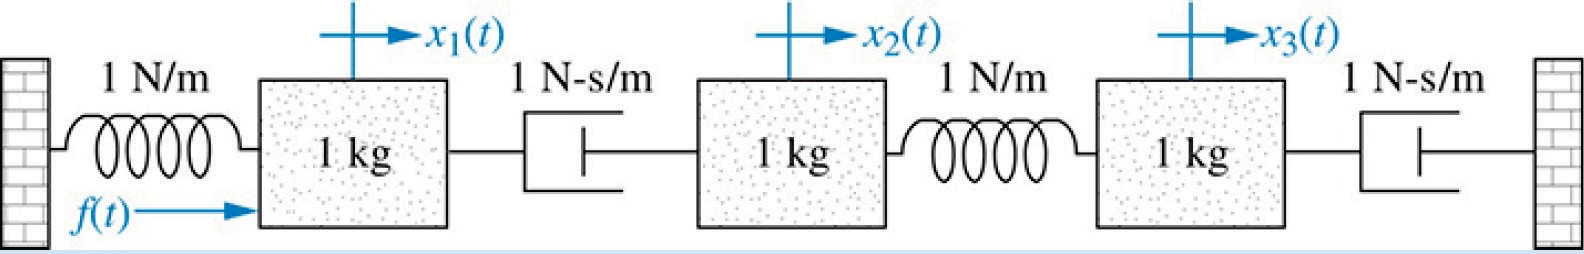
\includegraphics[width=\linewidth]{part01_translational_mechanical_system.png}
    \caption{Diagram of the translational mechanical system.}
    \label{fig:translational mechanical system}
\end{figure}

A state-space representation is a mathematical model of a physical system using variables that are in the time domain.

We are given the translational mechanical system in Fig. \ref{fig:translational mechanical system}. From this system, let's define masses
\begin{equation}
    \vec{M} := \brac*{
        \begin{matrix} M_1 & M_2 & M_3 \end{matrix}
    }^\transpose = \brac*{
        \begin{matrix} \SI1{\kilo\gram} & \SI1{\kilo\gram} & \SI1{\kilo\gram} \end{matrix}
    }^\transpose,
\end{equation}
spring constants
\begin{equation}
    \vec{K} := \brac*{
        \begin{matrix} K_1 & K_2 \end{matrix}
    }^\transpose = \brac*{
        \begin{matrix} \SI1{\newton\per\meter} & \SI1{\newton\per\meter} \end{matrix}
    }^\transpose,
\end{equation}
and damping constants
\begin{equation}
    \vec{D} := \brac*{
        \begin{matrix} D_1 & D_2 \end{matrix}
    }^\transpose = \brac*{
        \begin{matrix} \SI1{\newton\second\per\meter} & \SI1{\newton\second\per\meter} \end{matrix}
    }^\transpose.
\end{equation}

\addcontentsline{toc}{subsubsection}{Free body diagram}
This system has the free body diagram shown on the following CAD drawing.
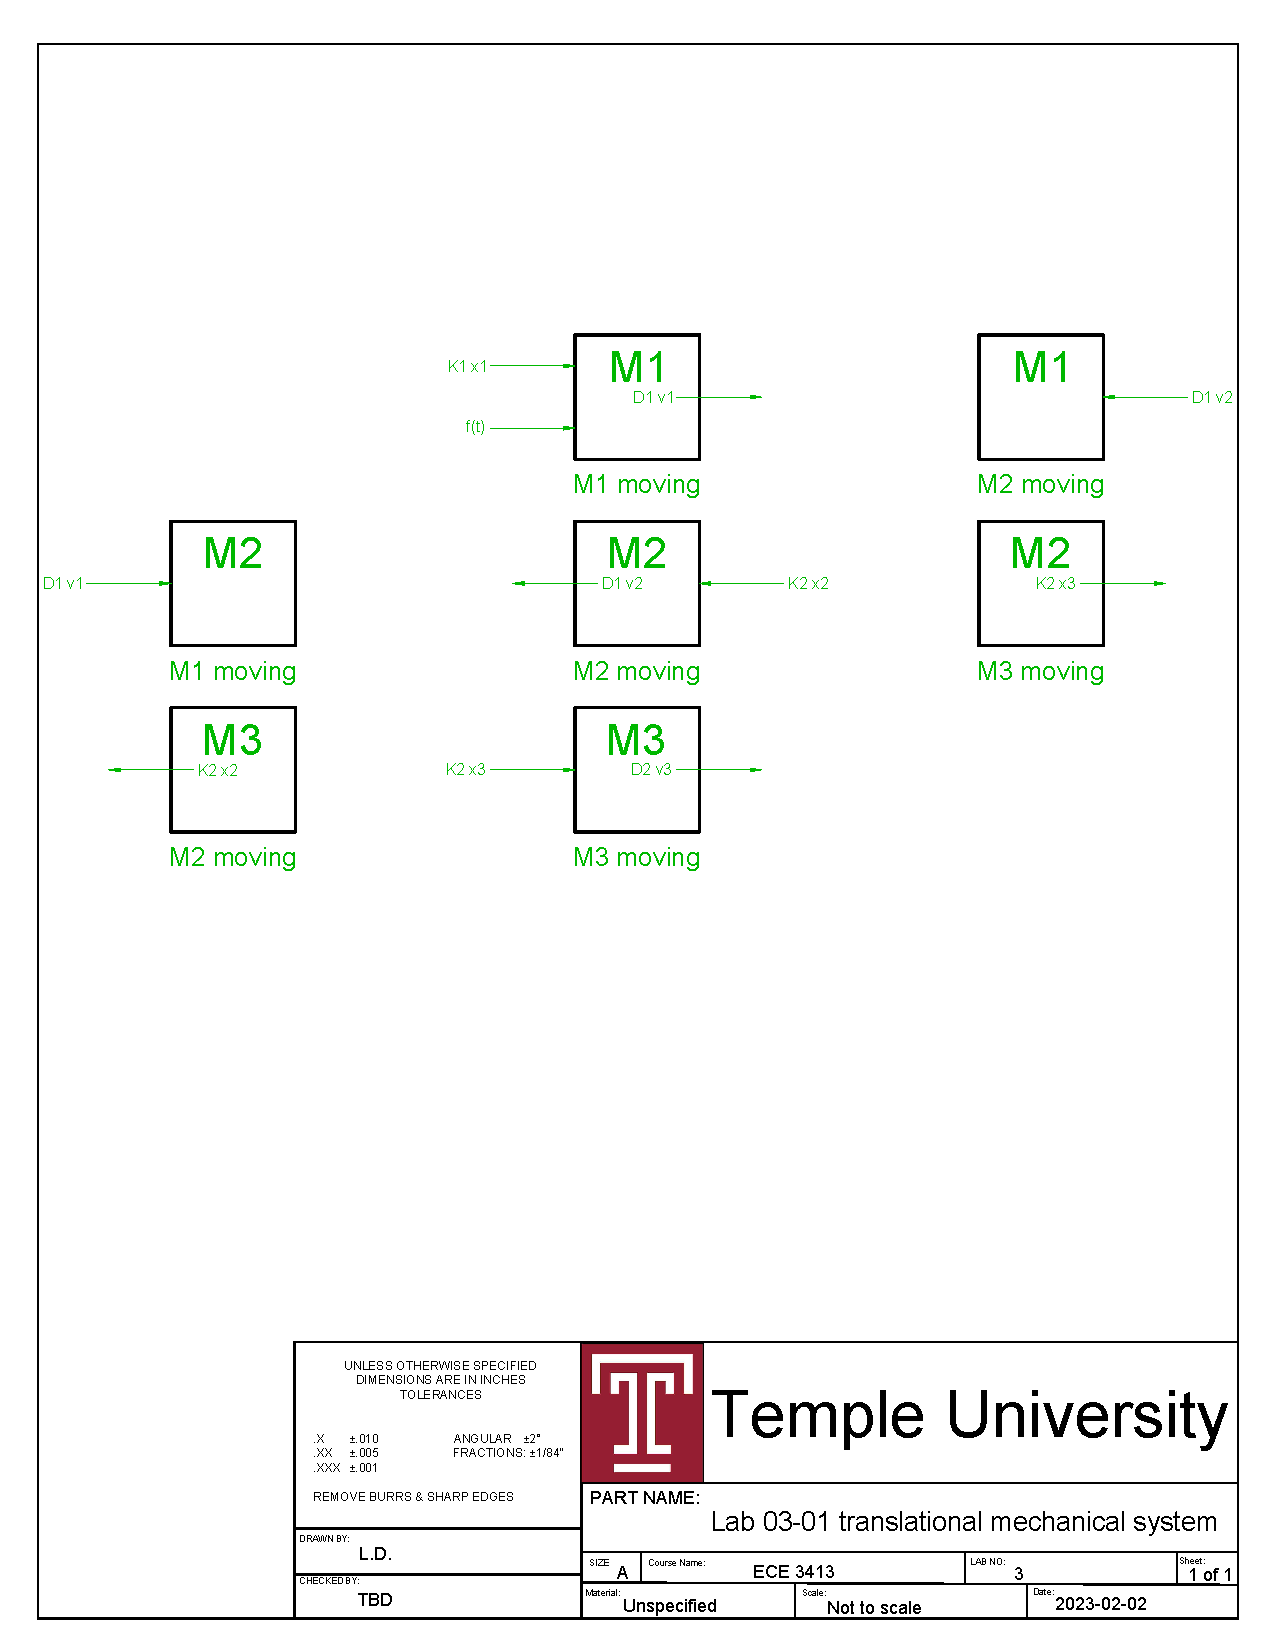
\includepdf{lab03-01 translational mechanical system fbd-A size.pdf}

\subsubsection{State-space representation}

Then we find the total force at each mass applying superposition for each possible state.

\begin{equation}
    \piecefn*{
        \begin{array}{@{}l@{}}
            M_1 \ddot{x}_1 = \sum F_{M1\mathrm{x}} = K_1 x_1 + f\brao*t + D_1 \brao*{\dot{x}_1 - \dot{x}_2},
        \\*
            M_2 \ddot{x}_2 = \sum F_{M2\mathrm{x}} = D_1\brao*{\dot{x}_1 - \dot{x}_2} + K_2\brao*{-x_2 + x_3},
        \\*
            M_3 \ddot{x}_3 = \sum F_{M3\mathrm{x}} = K_2\brao*{-x_2 + x_3} + D_2\dot{x}_3.
        \\*
        \end{array}
    }
\end{equation}

We relate position

\subsection{Roots and corresponding phase angles of a polynomial}

In this part of the lab, we model a polynomial in Matlab.
This is done by using a row vector.
Of the operations that can be performed on a row vector, $2$ are the \mintinline{matlab}{conv} and \mintinline{matlab}{roots} functions.

\subsubsection{Convolution}\label{sss:conv}

The \mintinline{matlab}{conv} function is used to convolve two vectors representing polynomial multiplication.

For example, we have the polynomials
\[
    \begin{gathered}
        P_1\brao*s = s^2 + 10s + 24\rlap, \\*
        P_2\brao*s = s^4 + 26s^3 + 231s^2 + 766s + 560\rlap. \\*
    \end{gathered}
\]

These may be represented by the row vectors
\[
    \begin{gathered}
        \vec{v}_1 := \brac*{\begin{matrix} 1 & 10 & 24 \\* \end{matrix}}\rlap, \\*
        \vec{v}_2 := \brac*{\begin{matrix} 1 & 26 & 231 & 766 & 560 \\* \end{matrix}}\rlap. \\*
    \end{gathered}
\]

\pagebreak

Then the convolution $\mathbf{v}_1 \ast \mathbf{v}_2$ represents the product $\brao{P_1 P_2}\brao*s$ as follows

\begin{minted}{matlab}
       [   1  26 231 766 560 ]
[ 24  10   1]                         = 1
    [ 24  10   1]                     = 10+26 = 36
        [ 24  10   1]                 = 24 + 260 + 231 = 515
            [ 24  10   1]             = 624 + 2310 + 766 = 3700
                [ 24  10   1]         = 5544 + 7660 + 560 = 13764
                    [ 24  10   1]     = 18384 + 5600 = 23984
                        [ 24  10   1] = 13440
-----------------------------------------------------------------
[1 10 24]*[1 26 231 766 560] = [1 36 515 3700 13764 23984 13440],
\end{minted}

representing the polynomial
\[
    P\brao*s = s^6 + 36s^5 + 515s^4 + 3700s^3 + 13764s^2 + 23984s + 13440\rlap.
\]

\subsubsection{The roots of the polynomial}

The \mintinline{matlab}{roots} function in Matlab returns the roots of the polynomial $P\brao*s$, that is, the values of $s$ s.t. $P\brao*s = 0$.

\subsection{Transfer functions}

In part 2 of the lab, we model a transfer function and modify one of its coefficients to produce a new output.

We use Matlab to set up the parameters for the transfer functions before using Simulink to model them because Matlab allows for a cleaner interface to set up the parameters.

Additionally, we can use Matlab to perform sanity checks along the way because it echos the value of every statement that is not suppressed by the semicolon character (\mintinline{matlab}{;}).

For example, we can echo the poles, zeros, numerators and denominators of the transfer functions to ensure that we set them up correctly.

Simulink is then used to model the system visually as a block diagram.
The transfer functions are compared by their step responses, their response to a step signal.
The signal starts at $\SI1\volt$, then jumpts to $\SI2\volt$ at $\SI1{\milli\second}$.

\subsubsection{Transfer functions in Matlab}

Matlab has transfer function objects.
These can be represented by objects as a ratio of polynomials using the \mintinline{matlab}{tf} function,
or as their zeros, poles and gain using \mintinline{matlab}{zpk}.
In this lab, we make use of the \mintinline{matlab}{tf} objects.

\subsubsection{Poles}

The poles are the roots of the denominator of the transfer function.
Matlab has the function \mintinline{matlab}{pole},
which accepts a transfer function and returns it poles.

\subsubsection{Zeros}

The zeros are the roots of the numerator of the transfer function.
Matlab has the function \mintinline{matlab}{zero},
which accepts a transfer function and returns it zero.

\subsubsection{The modified transfer function}

We are given the transfer function
\[
    H\brao*s = \frac{s^2 + 10s + 24}{s^4 + 26s^3 + 231s^2 + 766s + 560}\rlap.
\]

I have modified it by negating its pole with the minimum magnitude.

\section{Results}

\hr

%% This LaTeX was auto-generated from MATLAB code.
% To make changes, update the MATLAB code and export to LaTeX again.

\documentclass{article}

\usepackage[utf8]{inputenc}
\usepackage[T1]{fontenc}
\usepackage{lmodern}
\usepackage{graphicx}
\usepackage{color}
\usepackage{hyperref}
\usepackage{amsmath}
\usepackage{amsfonts}
\usepackage{epstopdf}
\usepackage[table]{xcolor}
\usepackage{matlab}

\sloppy
\epstopdfsetup{outdir=./}
\graphicspath{ {./part01_polynomials_mlx_images/} }

\begin{document}

\matlabtitle{Part 1 $-$ Roots and corresponding phase angles of a polynomial}


\matlabheading{Given the polynomial}

\begin{par}
$$P(s)=(s^2 +10s+24)(s^4 +26s^3 +231s^2 +766s+560),$$
\end{par}

\begin{matlaboutput}
P = 1x7    
           1          36         515        3700       13764 ...
           23984       13440

\end{matlaboutput}

\matlabheading{1. we find the roots of the resulting polynomial}

\begin{matlaboutput}
P_roots = 6x1    
  -10.0000
   -8.0000
   -7.0000
   -6.0000
   -4.0000
   -1.0000

\end{matlaboutput}

\matlabheading{2. and their corresponding phase angles}

\begin{matlabtableoutput}
{
\begin{tabular} {|c|c|c|}\hline
\mlcell{ } & \mlcell{P\_roots} & \mlcell{P\_root\_angles\_in\_deg} \\ \hline
\mlcell{1} & \mlcell{-10} & \mlcell{180} \\ \hline
\mlcell{2} & \mlcell{-8} & \mlcell{180} \\ \hline
\mlcell{3} & \mlcell{-7} & \mlcell{180} \\ \hline
\mlcell{4} & \mlcell{-6} & \mlcell{180} \\ \hline
\mlcell{5} & \mlcell{-4} & \mlcell{180} \\ \hline
\mlcell{6} & \mlcell{-1} & \mlcell{180} \\ 
\hline
\end{tabular}
}
\end{matlabtableoutput}
\end{document}


\ \hr \\*

This section is performed as a Matlab live script.

The polynomial convolved in Matlab is the same from subsubsection \ref{sss:conv}, and we found the expected resulting row vector of coefficients.

As for the roots, we also expected that the roots would have a phase angle of $\SI{180}\degree$,
which means that the roots would be a negative real number in the rectangular coordinate system.
The reason we expected these roots is because the polynomial has all positive coefficients.
This is one type of stable transfer function.

\subsection{Transfer functions}

\begin{figure}
    \centering
    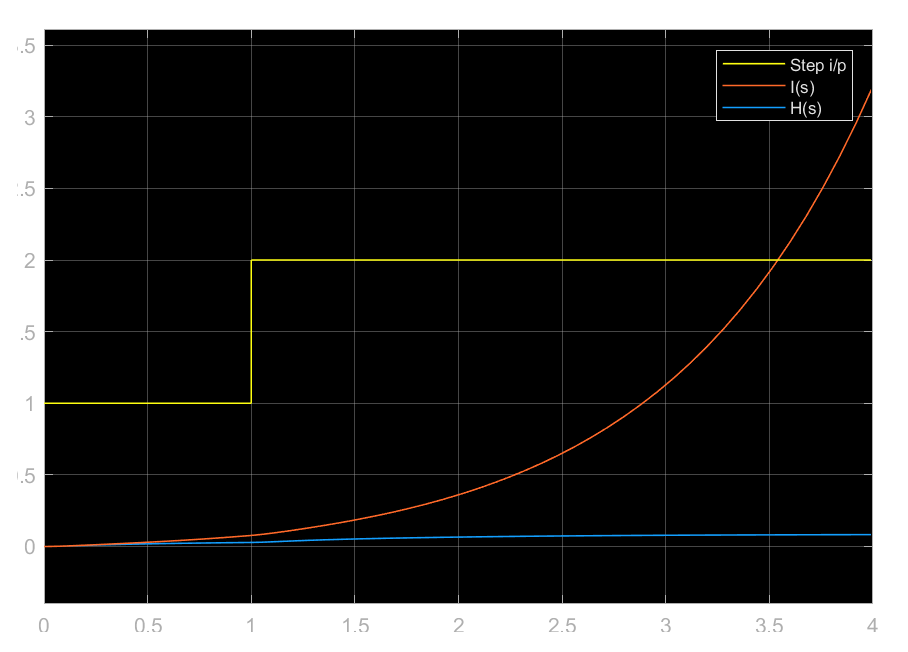
\includegraphics[width=\linewidth]{transfer_functions.eps}
    \caption{Modeling a simple input-output system, a stable step response and an unstable step response in voltage vs time in milliseconds.}
    \label{fig:transfer functions}
\end{figure}

\subsubsection{The roots and poles}

Given the transfer function 
\[
    H\brao*s = \frac{s^2 + 10s + 24}{s^4 + 26s^3 + 231s^2 + 766s + 560}\rlap,
\]
we find that the poles are in
\[
    \brac*{
        \begin{matrix}
            -10.0000 \\*
            -8.0000 \\*
            -7.0000 \\*
            -1.0000 \\*
        \end{matrix}
    }
\]
and the zeroes are in
\[
    \brac*{
        \begin{matrix}
            -6.0000 \\*
            -4.0000 \\*
        \end{matrix}
    }\rlap.
\]

Further, we modify this transfer function by negating the pole with the least magnitude ($-1.0000$) producing
\[
    I\brao*s = \frac{s^2 + 10 s + 24}{s^4 + 24 s^3 + 181 s^2 + 354 s - 560}\rlap.
\]

The result can be seen in Fig. \ref{fig:transfer functions}.

The step function jumps at $\SI1{\milli\second}$.
By $\SI3{\milli\second}$, $H\brao*s$ has settled at about $\SI1\volt$.
However, $I\brao{s}$ is at $\SI{1.129}\volt$ and goes beyond $\SI2\volt$ at time $\SI{3.543}{\milli\second}$.
It continues to grow exponentially.
This happens because $H\brao*s$ is a stable transfer function whereas $I\brao*s$ is unstable.

\section{Discussion}

This experiment was straightforward in its procedure.
We learned about how Matlab handles multiplication of polynomials,
and we also experienced a transfer function responding to a signal in a simulated system.

This experiment introduced the idea of stable and unstable transfer functions.
A stable transfer function can be used to attenuate a signal before it gets too far out of bounds.
However, an unstable function may not help with this.

Engineers may have more precise formulas to help choose the correct poles and zeros and properly design a transfer function.


\newpage
\appendix
\section{Appendix}
\subsection{Part 1 -- Roots and corresponding phase angles of a polynomial, Matlab Live Script}

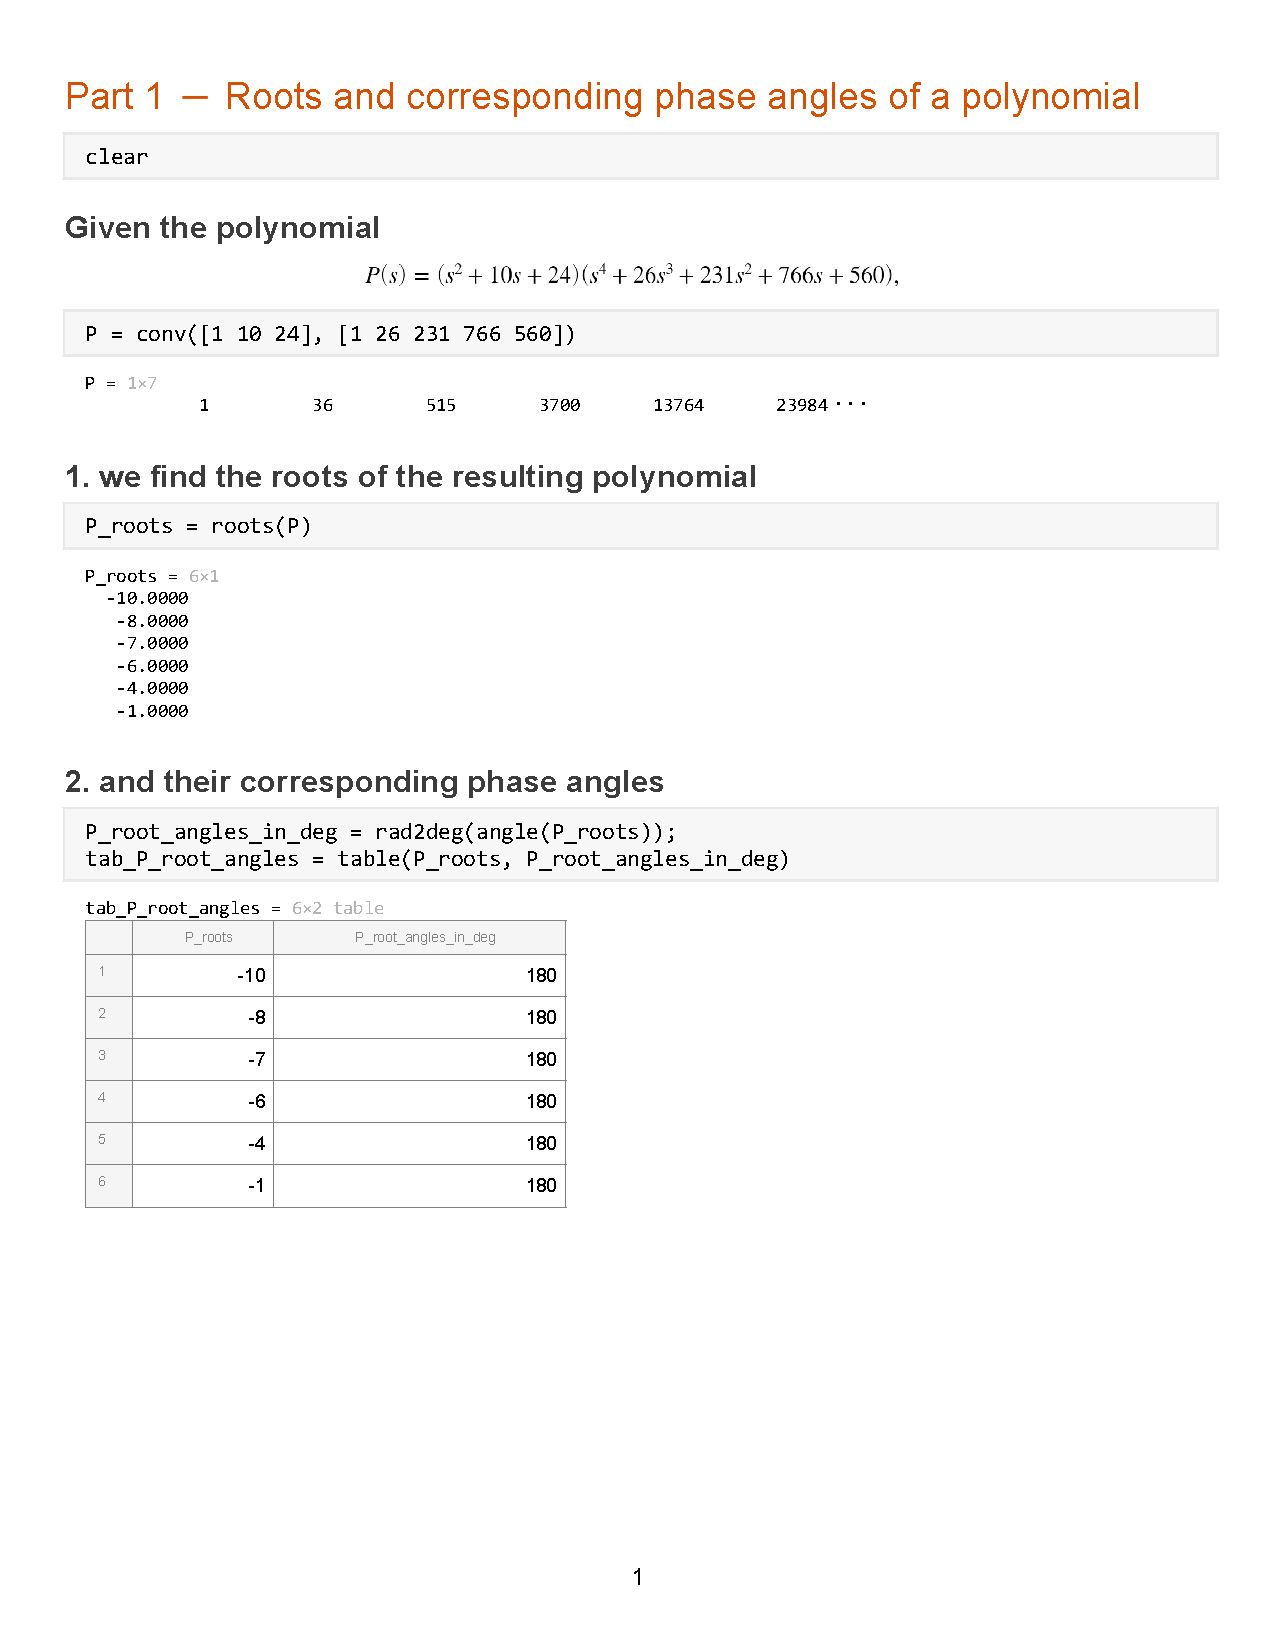
\includepdf{part01_polynomials_mlx.pdf}

\subsection{Part 2 -- Transfer function parameters}

\inputminted[]{matlab}{part02_01_transfer_function_params.m}

\subsection{Part 2 -- Modeling a system with a transfer function in Simulink}

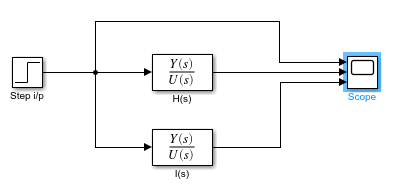
\includegraphics[width=\linewidth]{part02_02_modeling_transfer_function_system_slx.png}

\end{document}
